\chapter{EXE stage}
\label{chap:exe}

In this stage it is performed the actual instructions' execution and the load/store memory address calculation.
Its general block diagram is shown in figure \ref{fig:EXE_stage}.

\begin{figure}[!ht]
	\centering
	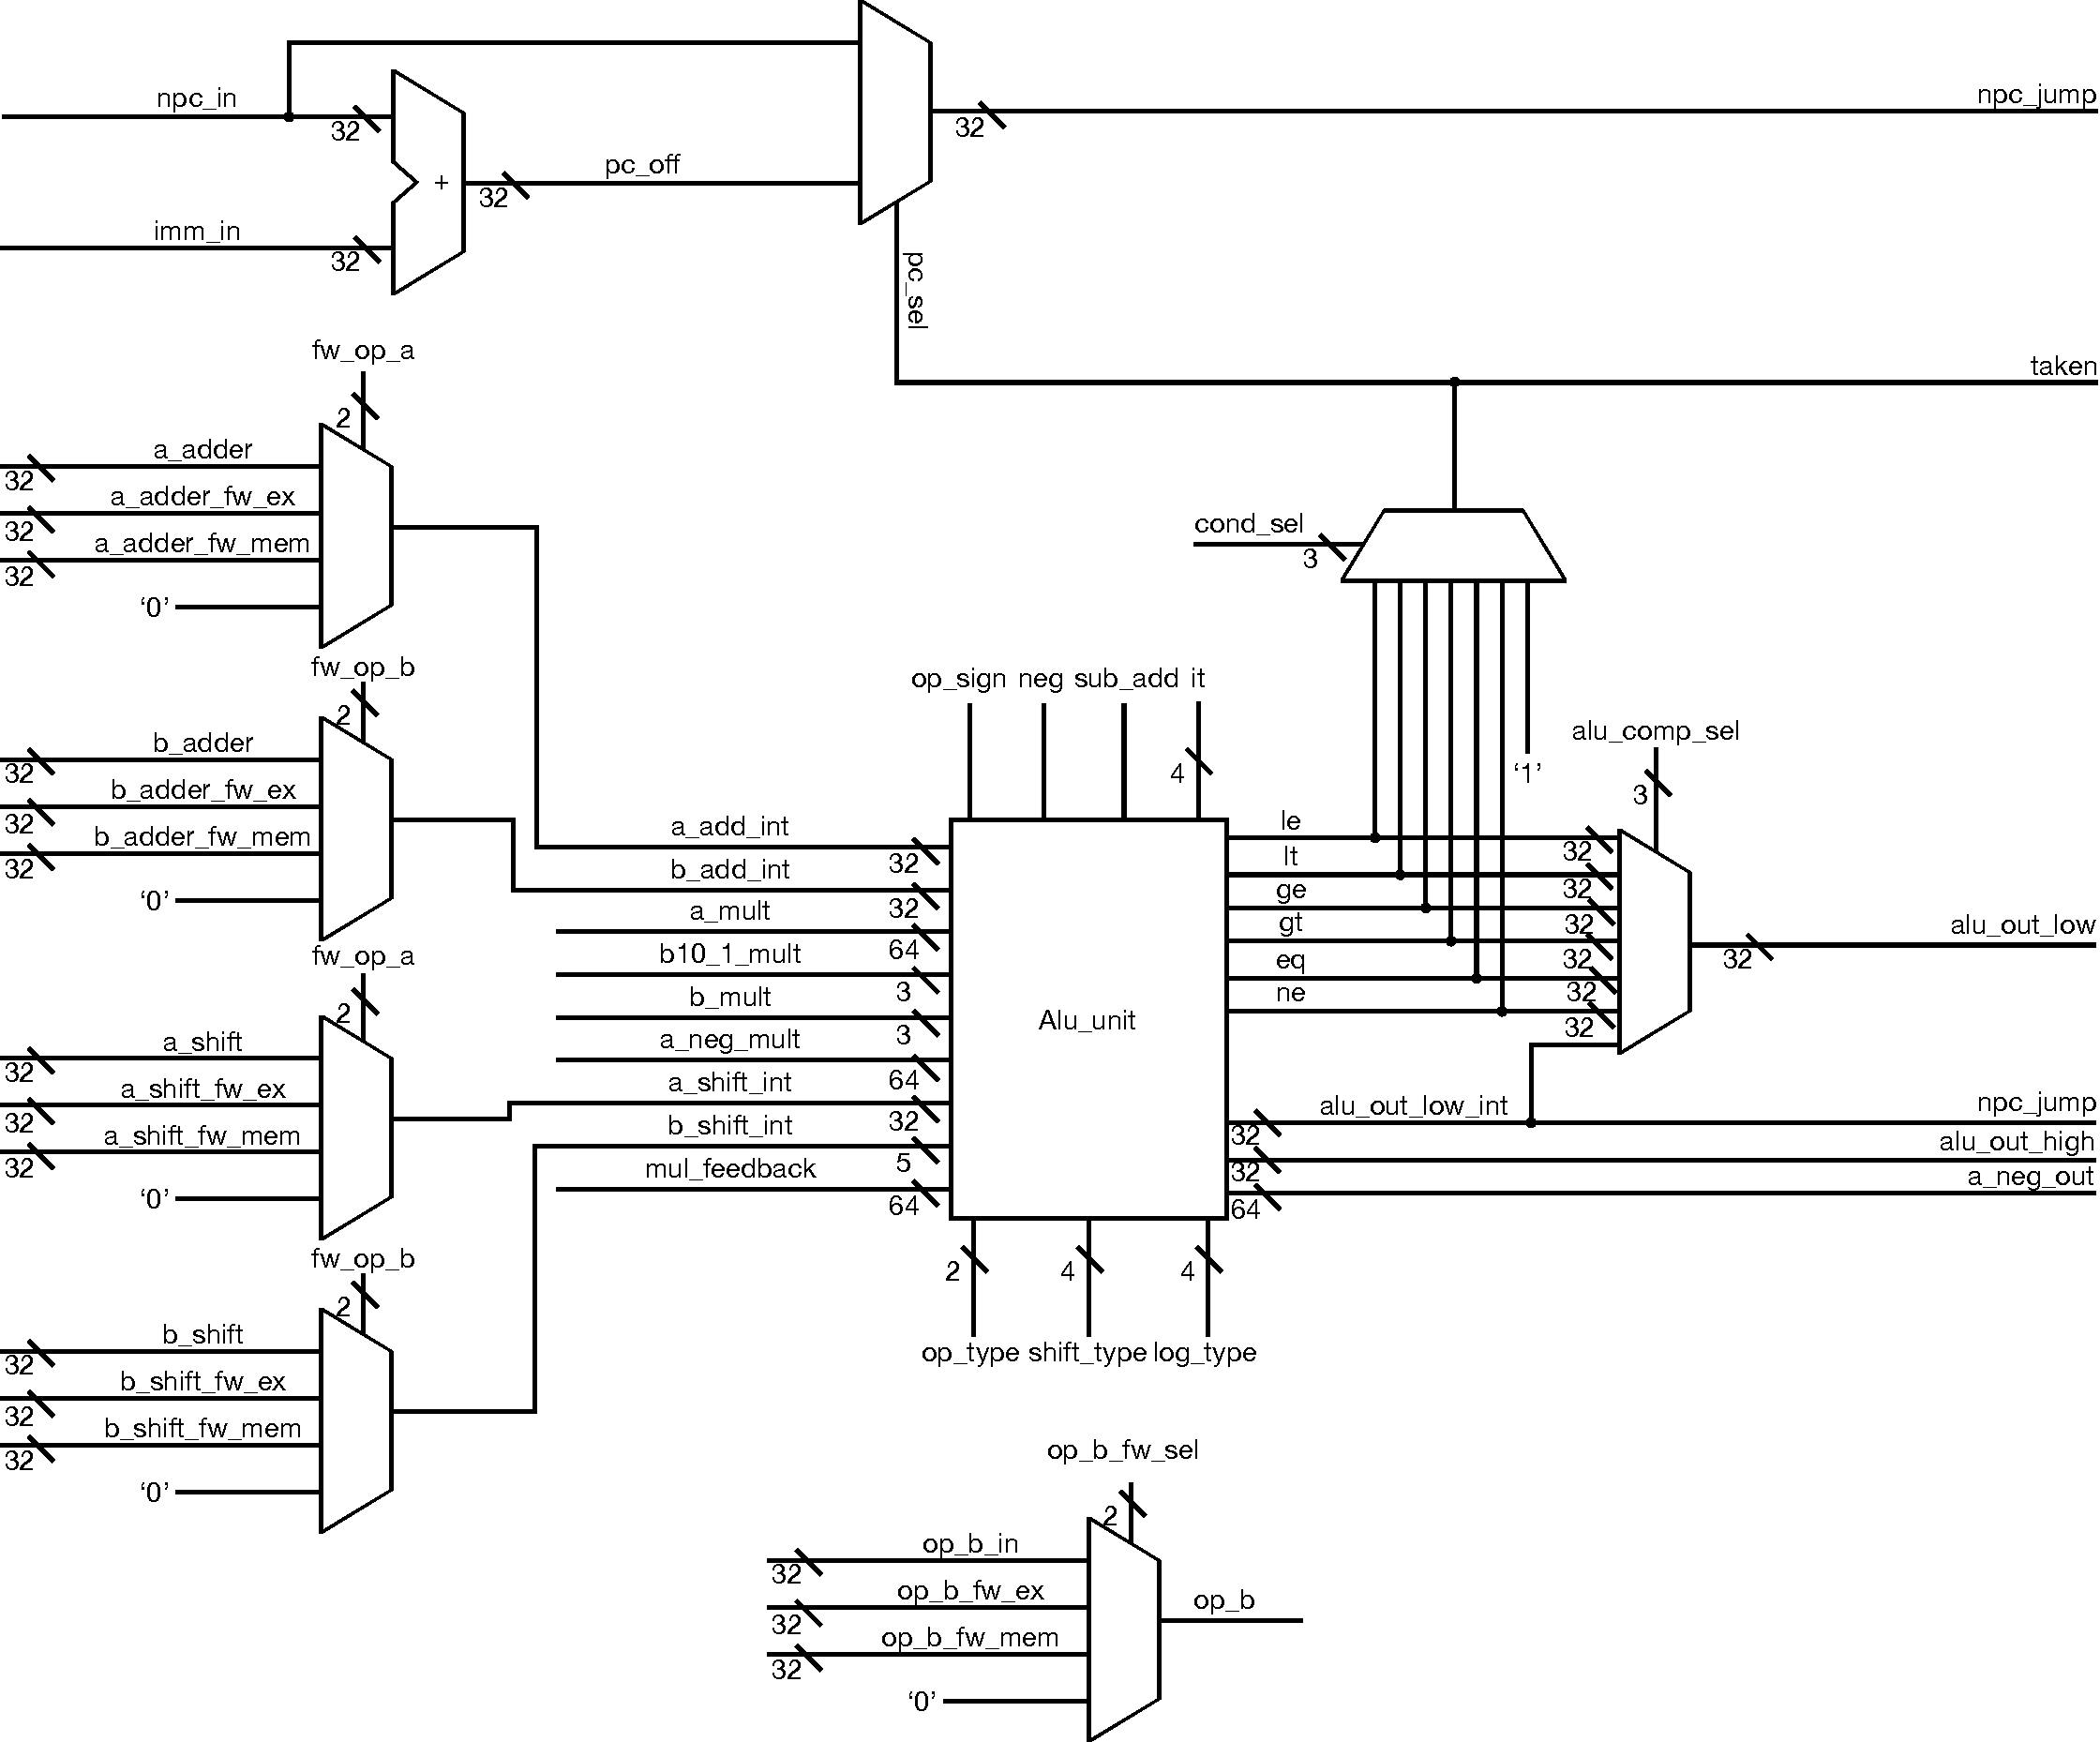
\includegraphics[width=0.8\linewidth]{./chapters/figures/ex_stage.pdf}
	\caption{Block diagram of the EXE stage}
	\label{fig:EXE_stage}
\end{figure}

The ALU incorporates the actual functional units, that are:

\begin{enumerate}
    \item an adder
    \item a shifter
    \item a logical unit
    \item a multiplier
\end{enumerate}

Each of these units have its own inputs coming from separate ID/EXE registers, the only exception being the adder and the logical units.
The rationale behind this is to reduce as much as possible the switching activity. These are, in fact, the most power hungry devices in the
whole datapath, therefore anything that can be done to reduce their power consumption leads to great benefits.

As it can be observed in the leftmost part of figure \ref{fig:EXE_stage}, the adder (and hence the logical), as well as the shifter, support forwarding.
Forwarding is also supported for the \verb|op_b| signal, that in case of a store contains the data to be written in cache.

At the center there is the ALU, discussed in details in section \ref{sec:alu}, and two muxes: the one that goes toward the top of the page is used to send
the \verb|taken| signal to the control unit in case of a branch execution and to drive the topmost mux, which outputs the correct value of the program counter.
The leftmost mux is, instead, used to select either the ALU's output signal or one of the internal comparator.

Finally, in the topmost part of figure \ref{fig:EXE_stage} there is a second adder, used to calculate $PC_{i+1} = PC_{i} + immediate$, where $i$ indicates the
current cycle number.

\section{ALU}
\label{sec:alu}

The ALU encapsulate, as said before, the various components that perform the wide range of supported operations. Its block diagram is shown in figure \ref{fig:alu}.

\begin{figure}[!ht]
	\centering
	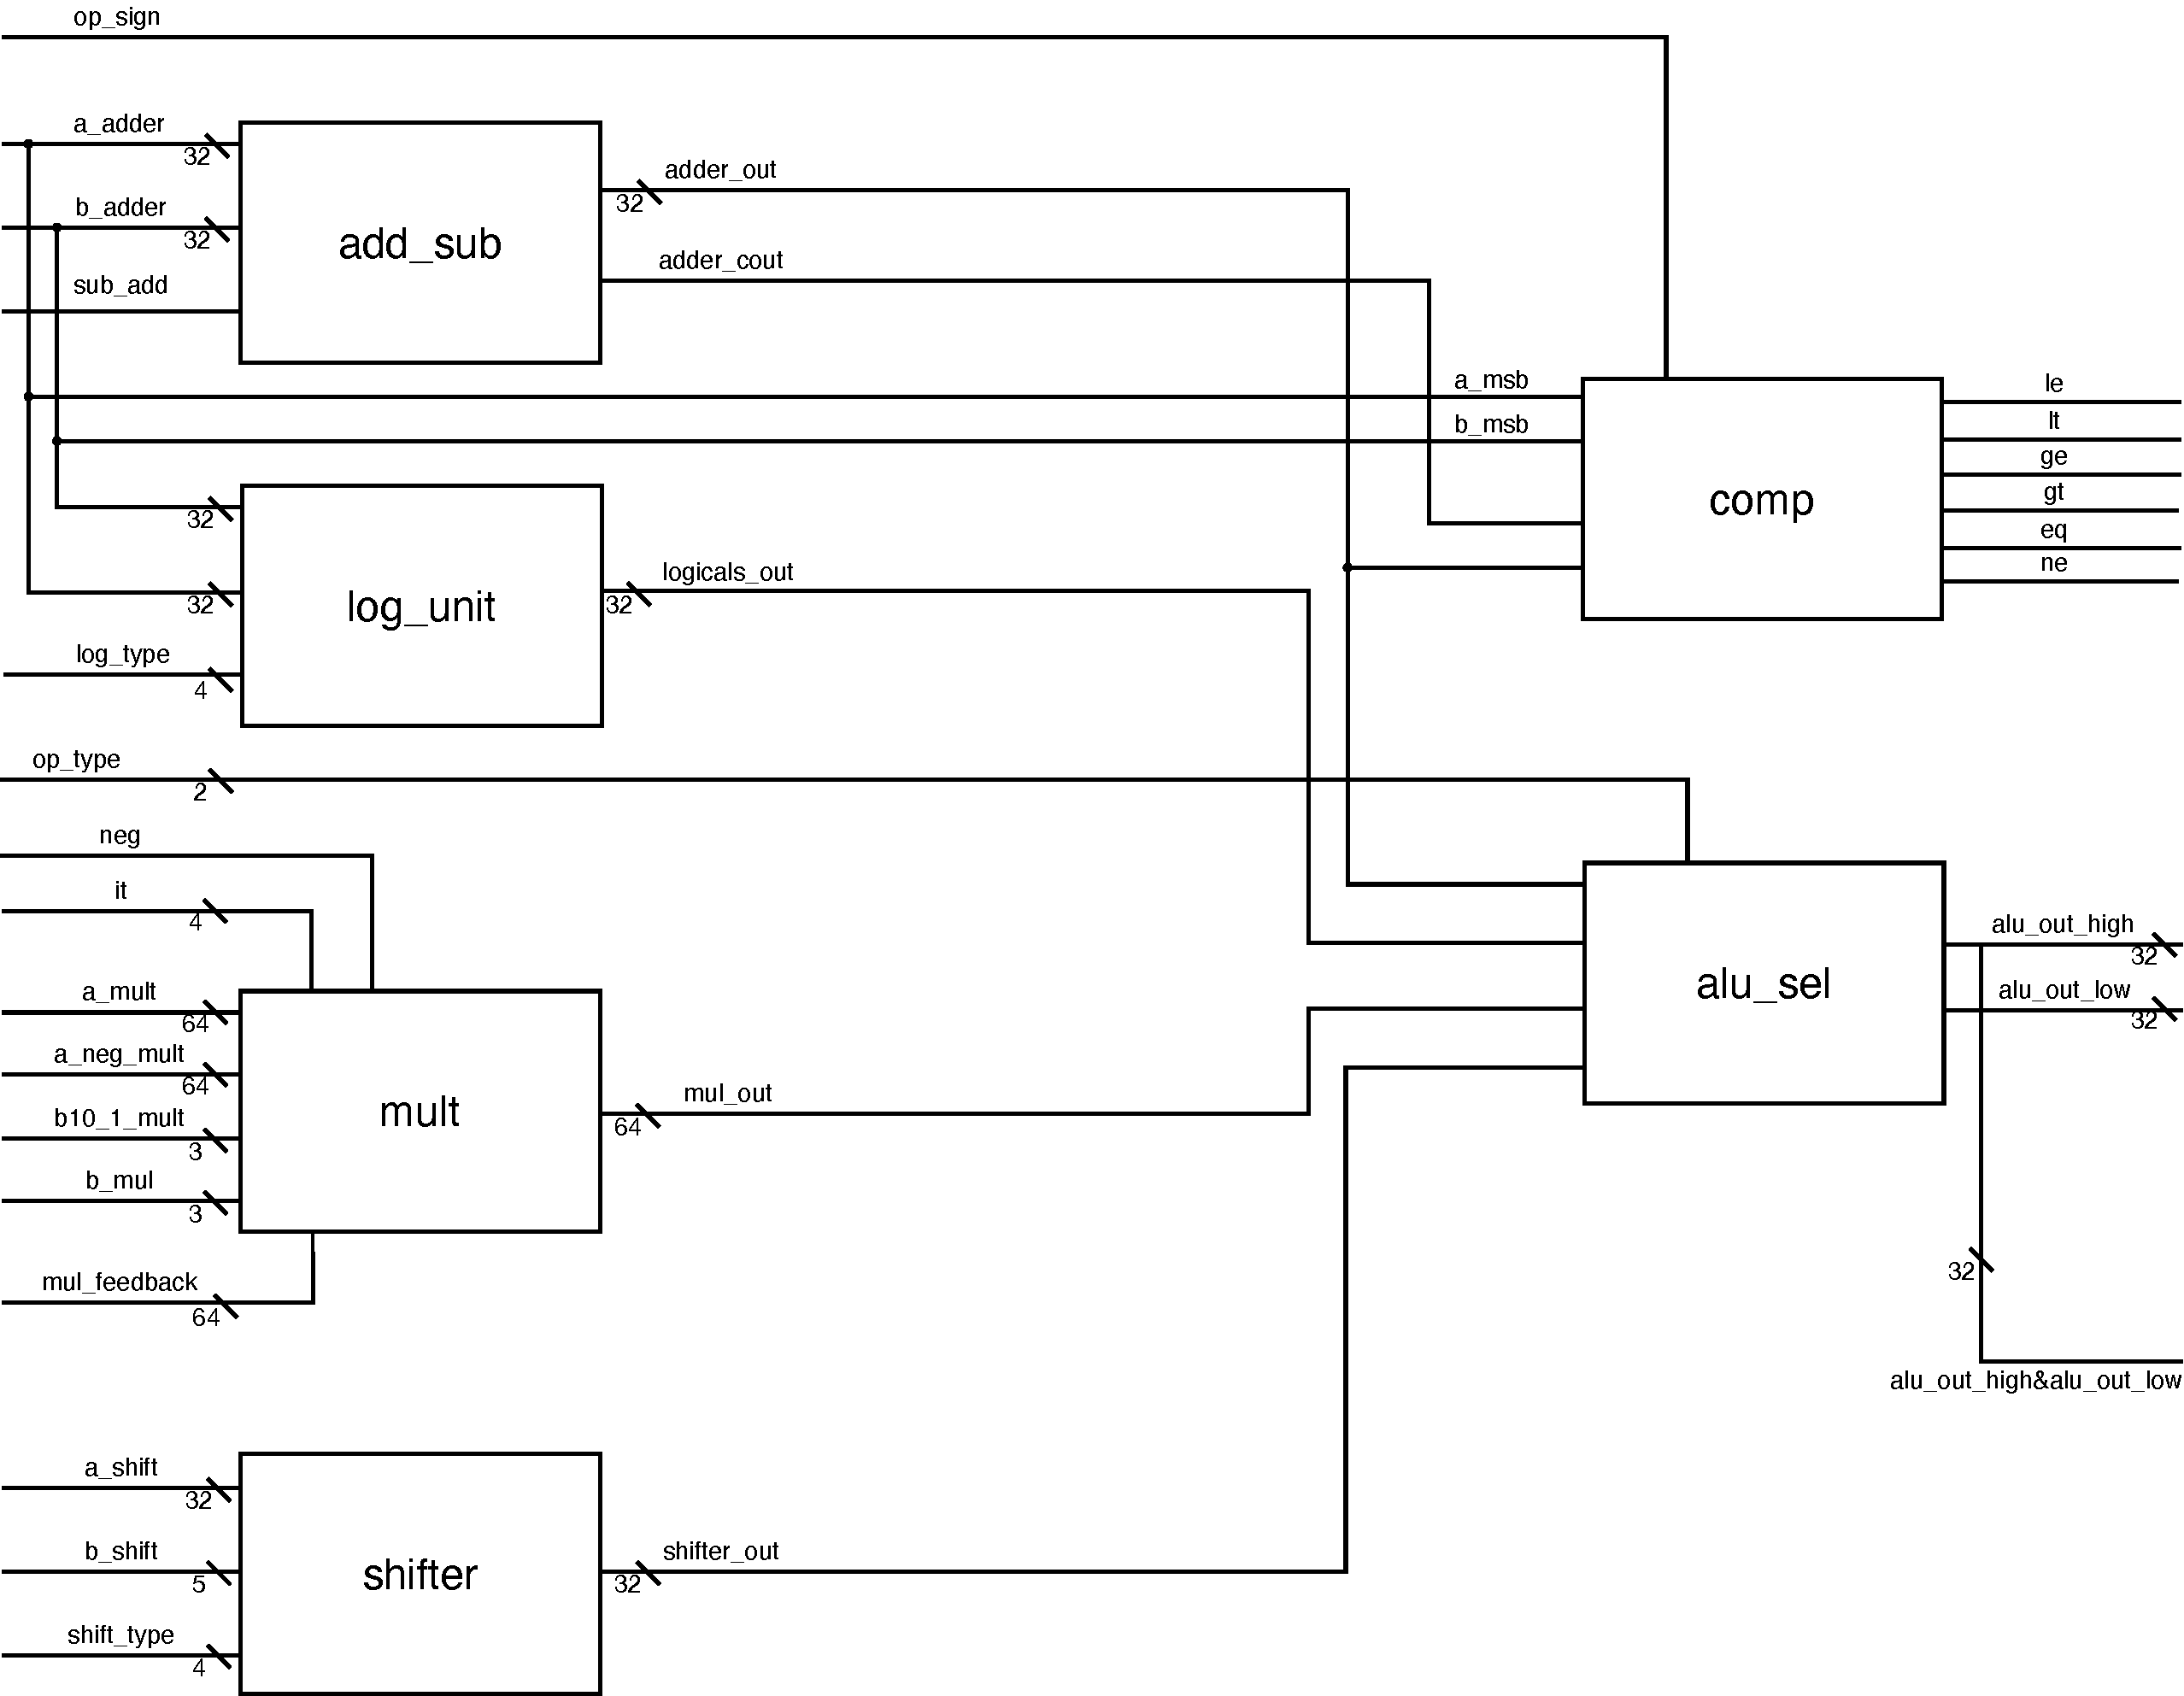
\includegraphics[width=0.8\linewidth]{./chapters/figures/ALU_exe.pdf}
	\caption{Block diagram of the ALU}
	\label{fig:alu}
\end{figure}

The adder, the logical unit and the shifter all implements structures seen during the lecture, in particular:

\begin{enumerate}
    \item the adder is an implementation of the P4.
    \item the logical unit implements the one seen inside the T2.
    \item the shifter is a smaller version than the one implemented in the T2.
\end{enumerate}

For this reason, for the various images and explanation of these units refer to \cite{ln}. 

\section{Branch \& Jump}